\documentclass[12pt, a4paper, twoside]{article}
\usepackage[margin=1in]{geometry}
\usepackage{times}
\usepackage{tabularx}
\newcolumntype{M}{>{\centering\arraybackslash}X}
\usepackage[hidelinks]{hyperref}
\usepackage{cite}
\usepackage{graphicx}
\graphicspath{ {assets/} }
\usepackage{float}
\usepackage{amsmath}
\usepackage[siunitx, RPvoltages, american]{circuitikz}
\usepackage{polyglossia}
\setdefaultlanguage{english}
\setotherlanguage{sanskrit}
\usepackage{fontspec}
\setmainfont{Times New Roman}
\newfontfamily{\devanagarifont}[Script=Devanagari]{Lohit Devanagari}
\newcommand{\Title}[1]{{\LARGE \centering \hrulefill\\ \textbf{#1}\\ \hrulefill}}
\date{}
\begin{document}
	\pagestyle{empty}
	\begin{titlepage}	
	\centering
	
	\LARGE A Seminar Report\\(MCS-291)\\on
	\vspace{1\baselineskip}
	
	\textbf{Emotionally Intelligent Machines \& Sentiment Synthesis based on Ancient Vedic Astrology}
	\vspace{1\baselineskip}
	
	
\includegraphics[width=150pt, keepaspectratio]{tmu_logo}
	
	College of Computing Sciences \& Information Technology\\Teerthanker Mahaveer University\\Moradabad
	\vspace{1\baselineskip}
	
	Submitted in partial fulfillment of	the requirements for the degree of \textbf{Master of Technology} by
	\vspace{1\baselineskip}
	
	\textbf{Mohit Singh\\(TCA-2212005)}
	\vspace{1\baselineskip}
	
	under the guidance of
	
	\textbf{Dr. Priyank Singhal} \& \textbf{Mr. Vikas Kuchhal}
	\vspace{1\baselineskip}
	
	{\Large \today}
\end{titlepage}
\clearpage
	\section*{\centering \LARGE Acceptance Certificate}
	\addcontentsline{toc}{section}{Acceptance Certificate}
	\vspace{1\baselineskip}
	\begin{tabularx}{\textwidth}{>{\hsize=0.5\hsize}XX}
	\begin{flushleft}
		
\includegraphics[width=150pt, keepaspectratio]{tmu_logo}
	\end{flushleft} & \begin{center}
		\vspace{2\baselineskip}
		\Large College of Computing Sciences \& Information Technology\\Teerthanker Mahaveer University\\Moradabad
	\end{center}
\end{tabularx}
\vspace{2\baselineskip}
 
\large The seminar report entitled ``Emotionally Intelligent Machines \& Sentiment Synthesis based on Ancient Vedic Astrology'' submitted by Mr. Mohit Singh (Enrollment No. TCA-2212005) may be accepted for being evaluated.
\vspace{2\baselineskip}

\begin{tabularx}{\textwidth}{XX}
	\begin{center}
		\textbf{Dr. Priyank Singhal}
	\end{center} & \begin{center}
	\textbf{Mr. Vikas Kuchhal}
\end{center} \\
	\begin{center}
		Signature\\ \today
	\end{center} & \begin{center}
	Signature\\ \today
\end{center} \\
\end{tabularx}
\clearpage
	\section*{\centering \LARGE Acknowledgements}
	\addcontentsline{toc}{section}{Acknowledgements}
	\vspace{1\baselineskip}
	\textit{``I would like to express my sincere gratitude to all those who have contributed to the completion of this research paper. Firstly, I am very grateful to my supervisors Dr. Priyank Singhal \& Mr. Vikas Kuchhal, my mentor Dr. Anu Sharma and jyotishachrya Mr. DK Lahori for providing me the guidance and support throughout the research. Their feedback, encouragement, and insightful comments have been invaluable in shaping this paper."}

\textit{``I am very grateful to Dr. RK Dwivedi the director of College of Computing Sciences \& Information Technology for providing me the opportunity to conduct this research as part of my academic program. This research has not only been a valuable learning experience but has also contributed to the knowledge base of the field."}

\textit{``I would also like to thank my colleagues and friends who provided me with valuable feedback and suggestions on the initial drafts of this paper. Their inputs have significantly improved the quality of this research."}

\textit{``Furthermore, I would like to express my gratitude to Teerthanker Mahaveer University for providing me the necessary resources and infrastructure to conduct this research. The library staff and resources have all played an integral role in the successful completion of this study."}

\textit{``The research skills and knowledge I have gained during my time at the college have been instrumental in shaping my approach to this research. I would also like to acknowledge the faculty members who have taught and mentored me during my academic journey, their insights and teachings have been invaluable in shaping my research skills and approach."}

\textit{``I am grateful to have had the opportunity to study at such an esteemed institution and to have been surrounded by individuals who have pushed me to achieve my best. Thank you, Teerthanker Mahaveer University, for contributing to my academic and personal growth."}

\textit{``Finally, I would like to thank my family for their unwavering support and encouragement throughout the research. Their love and understanding have been a source of strength and inspiration to me."}

\textit{``Once again, thank you to everyone who has contributed to this research."}
	\tableofcontents
	\newpage
	\pagestyle{plain}
	\Title{Emotionally Intelligent Machines \& Sentiment Synthesis based on Ancient Vedic Astrology}
	\section*{Abstract}
	\addcontentsline{toc}{section}{Abstract}
	After brain researchers have recognized that emotions are crucial for human and animal intelligence, Artificial Intelligence researchers have also started to acknowledge the importance of emotions in the design of intelligent machines. In this seminar, we will discuss about the Emotionally Intelligent Machines(EIM's) which is the new field of research in Artificial Intelligence but it has a great potential to do immense good, however the technology can be misused but it is up to the consumers of this technology who will decide whether it will be used for good or for evil. Also, Astrology has always been a controversial topic and is completely depends upto the personal faiths and beliefs of an individual. Apart from that, this paper describes that how Emotionally Intelligent Machines(EIM's) \& Sentiment Synthesis Systems can be developed by using the concept of Ancient Vedic Astrology.
	\section*{Keywords}
	\addcontentsline{toc}{section}{Keywords}
	Artificial Intelligence(AI), Emotional Intelligence(EI), Emotional Artificial Intelligence(EAI), Intution, Consciousness, Unconsciousness, Subconscious, Belief System, Feed Forward Network(FFN), Recurrent Neural Network(RNN), Convergence, Divergence,%Neural Networks, Sentimental Analysis, Vedic Astrology, Synthesis, Emotional Intelligence, Affective Computing, Subconsious, Cognitive Science, Philosophy, Psychology, Modalities, Galvanic Resistance, Bioinformatics, The Gateway Experience, Hemi-Sync, Cognitive Dissonance, Cognitive Harmony, Astral Travel, Hypnosis, Trasedental Meditation, BioFeedback(Creative Visualization), Emotion Dynamics
	\newline
	\hrule
	\section{Introduction}
	%For half a century, artificial-intelligence researchers have focused on giving machines linguistic and mathematical-logical reasoning abilities, modelled after the classic linguistic and mathematical-logical intelligences. This paper describes new research that is giving machines skills of emotional intelligence. Machines have long been able to appear as if they have emotional feelings, but they are now being programmed to also learn when and how to display emotion in ways that enable them to appear empathetic or otherwise emotionally intelligent. They are now being given the ability to sense and recognize expressions of human emotion such as interest, distress, and pleasure, with the recognition that such communication is vital for helping them choose more helpful and less-aggravating behaviour.

%Emotionally Intelligent Machines are the systems that can recognize, interpret, process, and simulate human emotions based on the concept of ancient vedic astrology. They are the machines which can adapt different situations and knows how to handle these situations more intelligently and smartly. In modern technical world, the need of EIM's are can be seen due to their numerous applications which are expanding rapidly. Some of the common applications of EIM's are:
	\section{Review of Literature}
	\begin{itemize}
	\item
	Need, Importance and benifits of Emotionally Intelligent Machines, What is Emotional Intelligence, Some applicaitons of EI, Limitations of Artificial Intelligence, \cite{ISSN-2456-2165}
	\item 
	
\end{itemize}
	\section{Theoretical Framework}
	\subsection{What is Artificial Intelligence?}
	Artificial Intelligence (AI) refers to the simulation of human intelligence in machines that are programmed to perform tasks that normally require human intelligence such as learning, problem-solving, decision-making, perception, language understanding, and more\cite{ISSN-2456-2165}. AI systems use algorithms and statistical models to analyze data, recognize patterns, and make predictions, without explicit instructions from human operators.

\subsubsection{Limitations of AI}
Although artificial intelligence (AI) has made significant advancements in recent years, there are still some limitations to the technology. Some of the limitations are:
\begin{itemize}
	\item \textbf{Lack of Common Sense:} AI systems lack the common sense that humans have, which can make it difficult for them to understand complex situations and make appropriate decisions.
	\item \textbf{Limited Creativity:} AI systems are designed to operate within the parameters set by their algorithms and data, which limits their ability to generate truly creative solutions or ideas.
	\item \textbf{Lack of Emotional Intelligence:} AI systems are not capable of experiencing emotions, which limits their ability to understand and respond to emotional cues in human interactions.
\end{itemize}
Limitations of AI highlight the need for continued research and development to address these issues and improve the capabilities of these systems.

	\subsection{What is Emotional Intelligence?}
	Emotional Intelligence (EI) refers to the ability to recognize, understand and manage one's own emotions as well as the emotions of others. It involves being able to use emotional information to guide thinking and behavior, and to navigate social situations effectively\cite{ISSN-2456-2165}.

EI is often described as having four components: self-awareness, self-management, social awareness, and relationship management. Self-awareness involves recognizing and understanding one's own emotions, strengths, and weaknesses. Self-management involves being able to regulate one's own emotions and behaviors in response to different situations. Social awareness involves recognizing and understanding the emotions of others, as well as the social norms and expectations of different situations. Relationship management involves using emotional information to communicate effectively, build and maintain relationships, and resolve conflicts.

EI is considered an important factor in personal and professional success, as it can help individuals navigate social interactions, build strong relationships, and manage stress and challenges effectively.
	\subsection{What is Emotional Artificial Intelligence?}
	Emotional Artificial Intelligence (EAI) is the ability of AI systems to recognize, understand, and respond appropriately to human emotions. It is an emerging field of AI that focuses on building machines that can perceive, interpret, and express emotions similar to human beings. 

Emotional AI uses various techniques such as natural language processing, sentiment analysis, and facial recognition to detect emotions in human interactions. These techniques are then used to train algorithms and models that can predict and respond to human emotions in real-time.

Emotional AI has numerous potential applications, such as improving customer service, enhancing human-robot interactions, and providing mental health support.
	\subsection{Why Truly Intelligent Machines Need Emotions?}
	Many machines are in our household items such as kitchen, bedroom, which are artificially intelligent to help us with our daily tasks, however, they are emotionally unintelligent to adapt to our fulfillment. If one desires an Artificial Intelligence, the Artificial Intelligence should be able to adapt to the individual's state of mind. At the present time, many leading companies have expanded the idea of Emotional Artificial Intelligence into their AI systems.\cite{ISSN-2456-2165}.

The need of EIM's are can be seen due to their numerous applications which are expanding rapidly.
Some of the common applications of EIM's include:
\begin{itemize}
	\item \textbf{Social Media:} They can be used in social media to analyse user's emotions and provide more personalized content.
	\item \textbf{Business Intelligence(BI) \& Operational Research(OR):} EIM's are more intelligent than the traditional machines as a result they can help in Decision Making which is involved in Business Intelligence \& Operational Research.
	\item \textbf{Human Resources:} In human resources to analyse employee's emotions and improve the work environment and productivity.
	\item \textbf{Development of Machine Ethics \& Computational Morality:} Emotional AI can play a vital role in the development of machine ethics and morality. It will allow machines to understand and respond to human emotions, which is an important component of ethical and moral decision-making.
	\item \textbf{Human-Computer Interaction(HCI):} Emotional AI is extremely helpful in HCI, as it enables computers to understand and respond to human emotions, making the interaction more natural, intuitive, and empathetic. Here are some ways in which Emotional AI can be useful in developing machine ethics and morality:
	\begin{itemize}
		\item \textbf{Understanding Human Emotions:} EAI can help machines to understand human emotions, which is an important component of ethical decision-making. For example, a machine that can detect when a human is experiencing fear or pain could adjust its behavior accordingly to avoid causing harm.
		\item \textbf{Ethical Decision-Making:} EAI can help machines to make more ethical decisions by taking into account human emotions and responses. For example, a self-driving car that can detect when a passenger is feeling anxious or stressed could adjust its driving style to provide a safer and more comfortable ride.
		\item \textbf{Morality and Empathy:} Emotional AI can help machines to exhibit more empathy towards humans, which is an important component of moral decision-making. For example, a robot that can detect when a human is feeling sad or lonely could provide comfort or companionship.
		\item \textbf{Human-Machine Collaboration:} Emotional AI can help facilitate collaboration between humans and machines by allowing machines to understand and respond to human emotions. This could lead to more effective and productive collaborations, as well as greater trust between humans and machines.
	\end{itemize}
	\item \textbf{Customer Service:} EAI can be used in customer service to understand customer's emotions and respond accordingly, improving customer satisfaction. It can also be used in getting customer reviews, feedbacks \& and conducting surveys.
	\item \textbf{Healthcare:} EAI could be very useful in healthcare sector to detect patient's emotions and provide appropriate treatment and care. They could be a great blessing for the treatment of psychic patients and for counselling of persons suffering form depression \& anxiety or even having suicidal tendency.
	\item \textbf{Education:} EAI can be used in education sector to improve the effectiveness of teaching by understanding the emotional state of the students and adapting the teaching method accordingly.
	\item \textbf{Marketing, Sales \& Advertisement:} EAI can be used in marketing to analyze customer's emotions and tailor marketing messages to maximize their impact which leads in increment of sales conversion rate.
	\item \textbf{Art \& Culture:} AI which can generate creative artistic content like Melodies \& Progressions in Music, Paintings \& Poetry is currently based on logical reasoning. By the development of Emotional AI, generation of this type of content can reach the next level of the arts which can also be used by the artists as a reference for their work.
	\item \textbf{Media \& Communication:} EAI has a huge potential to do great in the field of media as it can be used as a NEWS anchor or an interactive agent which can communicate with their listeners emoitionally.
	\item \textbf{Entertainment:} Emotionally Intelligent Machines can be used in the entertainment industry to create more immersive experiences for users by understanding their emotional responses, in gaming industry to create more engaging games that respond to the player's emotions also create the dynamic gaming environment accordingly, in movies industry to create ambience, environments and also in writing scripts.
\end{itemize}
	\subsection{Cognitive Psychology}
	Human mind is one of the most important part of the entire human body which contains thoughts, imagination, memory, will power \& sensation. Every human being has it's own personality. Some have similar personalities, some have not. The individual's own mindset is responsible for it's own personality and behaviour.

In psychology, according to Sigmund Freud, human mind is classified majorly into three categories. Conscious, subconscious \& unconscious mind. All the events around us which we are experiencing at the current instant which is also known as the "awareness", comes due to the conscious mind whereas all of our habits and routines which are formed due to the repetition of different task and our experiences are stored in the subconscious.
 
\begin{figure}[H]
	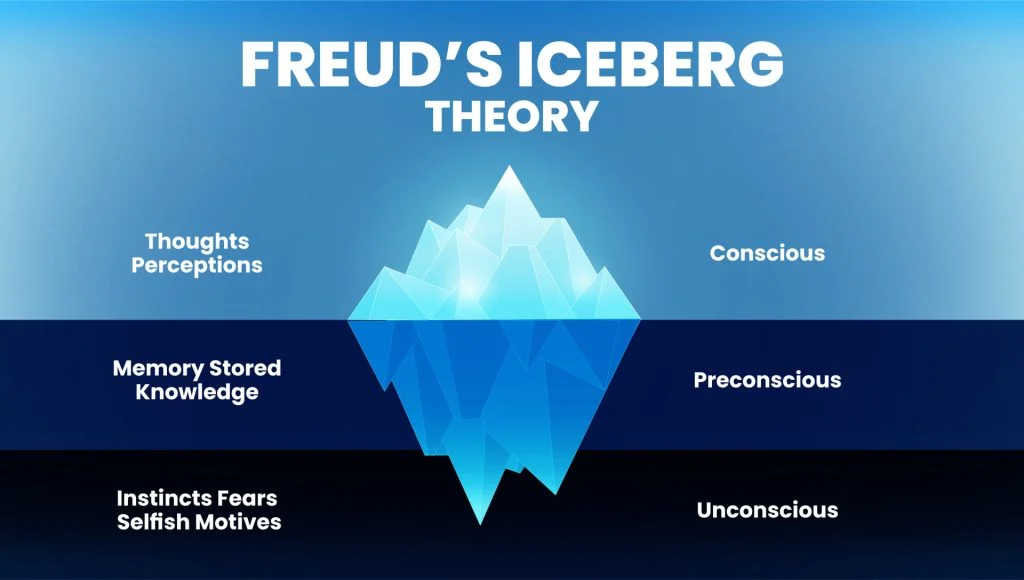
\includegraphics[width=\columnwidth, keepaspectratio]{FreudIcebergTheory}
	\caption{Sigmund Freud's Iceberg Theory}
	\label{Fig:fig1}
\end{figure}

The third type of category of mind is the most mysterious and powerful which is the unconscious mind. It operates beyond our conscious awareness. It is the part of our mind which contains thoughts, memories and emotions that we are not aware of, but that still influence our behaviour and feelings drastically. Conscious mind contains short-term memory. The content stored inside this type of mind can be changed easily on the other hand, the subconscious mind has long-term memory. It can store thoughts longer than the conscious mind which are difficult to change and involves practising something continuously, developing habits by doing continuous efforts in order to change the mindset. The unconscious mind has permanent memory which is almost impossible to be changed by any type of effort. It is the primary source of the human behaviour and personality. It is just like the default personality of a person. These three levels of mind can be understood by the Sigmund Freud's Iceberg Theory as shown in the figure \ref{Fig:fig1}.
	\subsection{Plutchik's Wheel of Emotions}
	Plutchik proposed a psychoevolutionary classification approach for general emotional responses.[2][3] He considered there to be eight primary emotions—anger, fear, sadness, disgust, surprise, anticipation, trust, and joy.
He also created a wheel of emotions to illustrate different emotions. Plutchik first proposed his cone-shaped model (3D) or the wheel model (2D) in 1980 to describe how emotions were related \cite{enwiki:1136521972}.
\begin{figure}[H]
	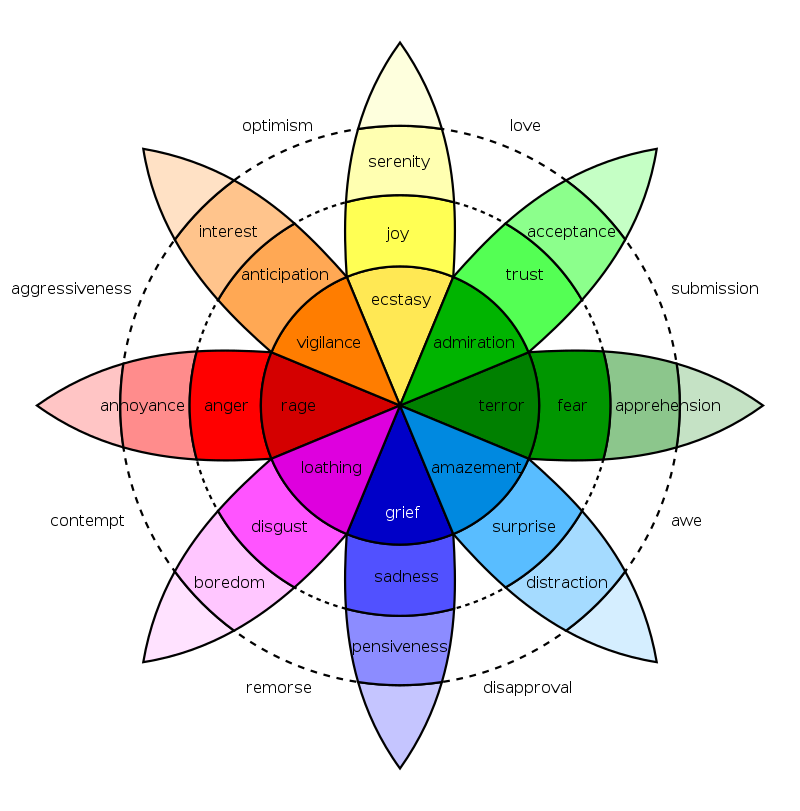
\includegraphics[width=\columnwidth, keepaspectratio]{Plutchik'sWheelofEmotions}
	\caption{Plutchik's Wheel of Emotions}
	\label{Fig:fig1}
\end{figure}
Figure \ref{Fig:fig1} shows PWOE.
\begin{figure}[H]
	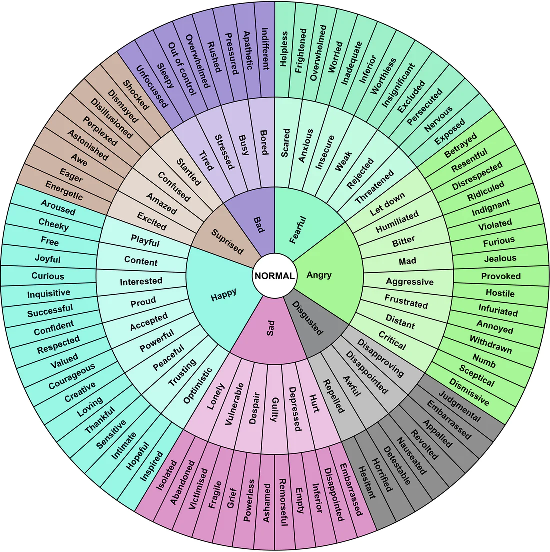
\includegraphics[width=\columnwidth, keepaspectratio]{PWOEEnglish}
	\caption{Full Plutchik's Wheel of Emotions English}
	\label{Fig:fig2}
\end{figure}
Figure \ref{Fig:fig2} shows  Full PWOE English.
\begin{figure}[H]
	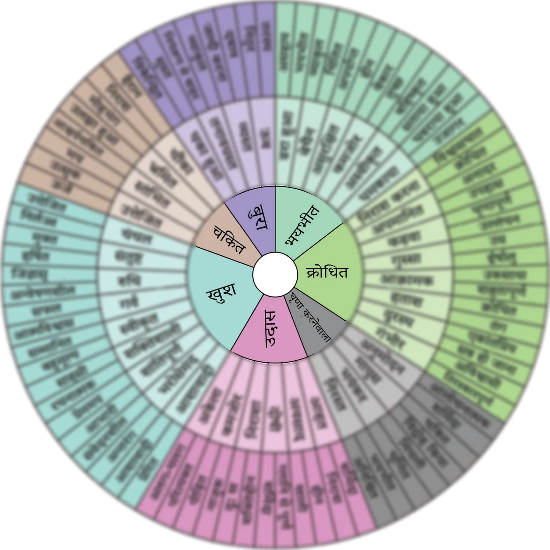
\includegraphics[width=\columnwidth, keepaspectratio]{PWOEHindi}
	\caption{Full Plutchik's Wheel of Emotions Hindi}
	\label{Fig:fig3}
\end{figure}
Figure \ref{Fig:fig3} shows PWOE Hindi.
	\subsection{Logical Thinking V/S Intuitive Thinking}
	Logic and intuition are two different ways of acquiring knowledge and making decisions. 

Logic is a systematic and rational way of thinking that relies on rules, principles, and evidence to arrive at a conclusion. It involves reasoning and analysis, and is based on the assumption that true knowledge can be acquired through objective observation and testing. Logical thinking is often associated with science, mathematics, and philosophy, and is used to solve problems and make decisions in a wide range of fields.

Intuition, on the other hand, is a more subjective and immediate way of knowing that is based on a person's instinct or "gut feeling" about a situation. It is often described as a kind of unconscious or automatic mental process that occurs without conscious awareness or reasoning. Intuitive thinking is associated with creativity, innovation, and quick decision-making, and is often used in fields such as art, design, and entrepreneurship.

While both logic and intuition can be useful in different contexts, they have different strengths and weaknesses. Logical thinking is often more reliable and accurate in situations where objective evidence and analysis are important, but it can be slow and cumbersome. Intuitive thinking is often faster and more flexible, but it can also be less reliable and more prone to bias and error. The most effective approach to problem-solving and decision-making often involves a combination of both logical and intuitive thinking, depending on the situation and the available information.
	\subsection{Emotion Dynamics}
	\begin{center}
	\begin{circuitikz}
		\draw (0,0) to[short] (0,2);
		\draw (0,2) to[L=$L(Craving)$, i>_=$i(t)$] (3,2);
		\draw (3,2) to[R=$R(Anger)$, i>_=$i(t)$] (6,2);
		\draw (6,2) to[C=$C(Attachment)$, i>_=$i(t)$] (9,2);
		\draw (9,2) to[short] (9,0);
		\draw (9,0) to[vsource, v=$v(t)(Will Power)$] (0,0);
	\end{circuitikz}
\end{center}
\begin{equation}
	\boxed{v(t) = L\frac{di(t)}{dt} + Ri(t) + \frac{1}{C}\int i(t)dt}
\end{equation}
	\subsection{Butterfly Effect \& Chaos Theory}
	Richard A. Anthes in 2022 by his paper ``Predictability \& Predictions" showed his experiences with predictability theory and weather predictions began as an undergraduate student at the University of Wisconsin in Madison in the early 1960s. His interest in numerical simulations led to the development of a simple nonlinear one-dimensional gravity wave model and later a nonlinear, baroclinic, three-dimensional model of the tropical cyclone. His experiences highlighted the challenges of numerical and physical instabilities in weather prediction models\cite{atmos13081292, encyclopedia2030084}.
In chaos theory, the butterfly effect is the sensitive dependence on initial conditions in which a small change in one state of a deterministic nonlinear system can result in large differences in a later state.
	\subsection{Long-Short Term Memory(LSTM)}
	Long Short-Term Memory (LSTM) is a type of recurrent neural network (RNN) architecture that has gained significant popularity in the field of deep learning. It addresses the limitations of traditional RNNs in capturing long-term dependencies by introducing a memory cell that allows the network to retain information over long sequences.

LSTM networks were introduced by Hochreiter and Schmidhuber in 1997 and have since become a fundamental component in various applications, particularly in natural language processing, speech recognition, and time series analysis\cite{article}.

\begin{figure}[H]
	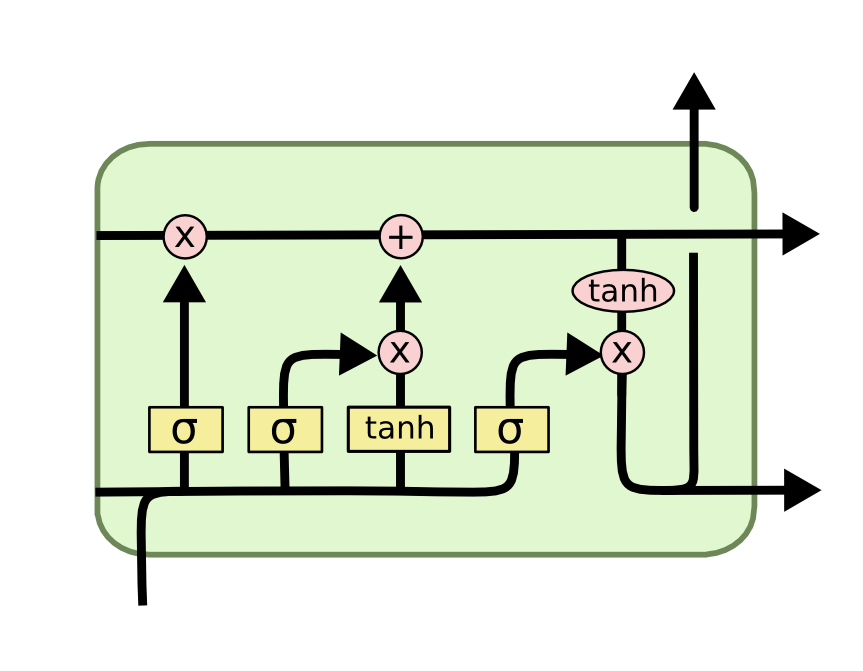
\includegraphics[width=\columnwidth, keepaspectratio]{LSTMChain}
	\caption{LSTM as Conscious \& Subconscious of AI}
	\label{Fig:fig4}
\end{figure}

The LSTM architecture consists of several specialized gates that control the flow of information as show in figure \ref{Fig:fig4}. These gates include the input gate, forget gate, output gate, and cell update gate. Each gate is composed of a sigmoid activation function, which determines the amount of information to be passed through. If we observe the working of the LSTM-RNN, we can understand that when a sequential data pattern repeats frequently, the LSTM stores it in a separate cell known as the memory cell$ (c_{t-1}) $ present within its architecture, just like the human subconscious mind forms habits by performing consciously repeating actions and patterns of life.
	\subsection{Vedic Astrology}
	Astrology is like the snapshot of our unconscious mind. The planetary vibrations reflected or refracted along with solar radiations to the earth are of varying intensities as per planetary distance, size, and movement in the solar system. These vibrations impact our sensory nerves, mental attitudes, and moods. Thus, it’s very likely that these planetary vibrations supply the energies to the body cells though our nerves. Since these vibrations differ in wavelength intensity and frequency as per the planetary properties and motion. These vibrations supply different sensory stimuli which impacts the human unconscious and personality at the time of birth\cite{article1}.

\subsubsection{Classification of Vedic Astrology}
Vedic astrology, also known as Jyotish, is an ancient system of astrology that originated in the Indian subcontinent. It is considered one of the oldest astrological systems in the world and has its roots in the Vedas, the ancient sacred texts of Hinduism.
Vedic astrology(Jyotish) is one of the most important limb(Vedanga) out of the total six limbs(Vedangas) found in the ancient Indian scriptures. The origins of Vedic astrology can be traced back to around 1500 BCE, during the late Vedic period. It is classified into the three major branches or disciplines known as the Siddhanta, Samhita and Hora. These branches provide different approaches and methods for studying and practicing astrology.

\begin{itemize}
	\item \textbf{Siddhanta:} Siddhanta deals with all the mathematical calculations of space \& time which is involed in the study of planets, stars, comets and contellations present in the space. It is also referred as the Astronomy in modern days.
	\item \textbf{Samhita:} Samhita, also known as Muhurtha, is the branch of Vedic astrology that deals with collective or mundane astrology. It focuses on predicting and analyzing events and phenomena on a broader scale, such as natural disasters, weather patterns, political developments, and societal events.
	\item \textbf{Hora:} Hora or horarian astrology is the branch of Vedic astrology that specifically deals with individual horoscopes or birth charts (Jataka).
\end{itemize}

There are many ancient texts and scriptures about all these three branches of the vedic astrology, that were written by Maharishies. But here, we are only considering the Surya Siddhanta\cite{SuryaSiddhanta, wiki:ss} and Brihat Parashara Hora Shastra\cite{BrihatParasharHoraShastraVol1, BrihatParasharHoraShastraVol2, wiki:bphs} which are the most popular texts that are used by most of the astrologers today for astrological predictions and consultations. We also discuss some of rules and priciples described by the dictums found in these texts.

\subsubsection{Properties of Planets}
The study of planets holds great significance in understanding an individual's horoscope and predicting future events. Vedic astrology recognizes nine celestial bodies as planets, including the Sun, Moon, Mercury, Venus, Mars, Jupiter, Saturn, Rahu, and Ketu. Each planet's placement, aspects, and interactions with other planets in an individual's birth chart play a crucial role in determining their personality traits, strengths, challenges, and life events according to Vedic astrology. Here's a brief introduction to each of these planets in the context of Vedic astrology:

\begin{itemize}
	\item \textbf{Sun (Surya):} The Sun represents the self, vitality, authority, and leadership. It symbolizes the soul and is considered the king among the planets.
	\item \textbf{Moon (Chandra):} The Moon represents emotions, mind, instincts, and nurturing qualities. It influences the individual's emotional well-being and intuition.
	\item \textbf{Mercury (Budha):} Mercury is associated with communication, intellect, logic, and adaptability. It governs speech, learning, and mental abilities.
	\item \textbf{Venus (Shukra):} Venus is the planet of love, beauty, art, and harmony. It governs relationships, attraction, creativity, and material pleasures.
	\item \textbf{Mars (Mangal):} Mars signifies energy, passion, courage, and assertion. It governs ambition, drive, physical strength, and competitiveness.
	\item \textbf{Jupiter (Guru):} Jupiter is considered the most benefic planet in Vedic astrology. It represents wisdom, knowledge, expansion, abundance, and spirituality.
	\item \textbf{Saturn (Shani):} Saturn is associated with discipline, responsibility, hard work, and karmic lessons. It teaches patience, endurance, and signifies limitations and life challenges.
	\item \textbf{Rahu:} Rahu is a shadow planet and represents material desires, obsession, illusions, and worldly attachments. It signifies ambition and can bring sudden changes.
	\item \textbf{Ketu:} Ketu is the other shadow planet and represents spirituality, detachment, mysticism, and karmic lessons. It signifies liberation and can bring unconventional experiences.
\end{itemize}

\subsubsection{Dashas \& Transits}
In Vedic astrology, dashas and transits are important techniques used to predict and analyze various aspects of a person's life based on the positions of planets and their movements at particular time periods after the birth of an individual. Chapter 53 of BPHS\cite{BrihatParasharHoraShastraVol1, BrihatParasharHoraShastraVol2, wiki:bphs} discusses about different effects of dashas of the different planets.

\begin{itemize}
	\item \textbf{Dashas:} Dashas are planetary periods that determine the major themes and influences in a person's life. They are calculated based on the position of the Moon at the time of birth. Each dasha is associated with a specific planet, and it represents a specific time period during which that planet's energy dominates. The most commonly used dasha system is the Vimshottari Dasha, which consists of a cycle of major and sub-periods of the planets.
	\item \textbf{Transits:} Transits, also known as `gochara', refer to the current positions of planets in relation to an individual's birth chart. They provide insights into the ongoing influences and events happening in a person's life. The movement of planets in the sky affects different areas of life and can trigger various experiences and opportunities. Astrologers analyze transits to understand the potential effects of planetary movements on different aspects of life, such as career, relationships, health, and finance. Table \ref{Table:table} represents the time required by all nine planets to complete one zodiac sign which is calculated in chapter 1, verse 29 to 34 of Surya Siddhanta\cite{SuryaSiddhanta, wiki:ss}.
\end{itemize}

\noindent
\begin{table}[H]
	\begin{tabularx}{\columnwidth}{|M|M|M|}
		\hline
		\textbf{Graha(Planet)} & \textbf{Angular Speed(\textdegree/Day)} & \textbf{Time For One Zodiac Sign} \\
		\hline
		Surya(Sun) & 1 & 1 Month \\
		\hline
		Chandra(Moon) & 13 & 2.25 Days \\
		\hline
		Brihaspati(Jupiter) & 1/12 & 1 Year \\
		\hline
		Shani(Saturn) & 1/30 & 2.5 Years \\
		\hline
		Budh(Mercury) & 1 & 1 Month \\
		\hline
		Shukra(Venus) & 1 & 1 Month \\
		\hline
		Mangal(Mars) & 2/3 & 1.5 Month \\
		\hline
		Rahu & -1/18 & 18 Months \\
		\hline
		Ketu & -1/18 & 18 Months \\
		\hline
	\end{tabularx}
	\caption{Time required by all planets to complete one zodiac sign}
	\label{Table:table}
\end{table}

Dashas and transits are used together to gain a comprehensive understanding of a person's life events and their timing. Dashas provide long-term trends and major life themes, while transits offer more immediate influences and shorter-term predictions. By analyzing the interaction between the dashas and transits, astrologers can make predictions, provide guidance, and suggest remedies to navigate through life's challenges and make the most of favorable periods.
	\section{Conclusion \& Outlook}
	The human mind is a very complex dynamical system that evolves over time in responses to the various inputs from the environment. The more we attempt to understand it deeply, the more we find ourselves entangled in questions. However, this pursuit provides us with new knowledge that leads to innovation and presents numerous challenges. The study of the human mind has been instrumental in the birth of artificial intelligence (AI), but there still exists a significant difference between AI and the human mind. To bridge this gap, psychology and Vedic astrology can play a crucial role, and by leveraging these theories, intuition-based AI systems could be developed in the future.
	\hrule
	\bibliography{Citations}
	\bibliographystyle{ieeetr}
	\section*{Appendix}
	\addcontentsline{toc}{section}{Appendix}
	\appendix
	\listoftables
\listoffigures
\section{\\Title of Appendix A}
% the \\ insures the section title is centered below the phrase: AppendixA

Text of Appendix A is Here

\section{\\Title of Appendix B}
% the \\ insures the section title is centered below the phrase: Appendix B

Text of Appendix B is Here
\end{document}